\documentclass[a4paper,11pt]{article}
\usepackage[slovene]{babel}
\usepackage[utf8]{inputenc}
\usepackage[T1]{fontenc}
\usepackage{lmodern}
\usepackage{amsmath, amsthm, amsfonts, amssymb}
\usepackage{graphicx}
\usepackage{float}

%%%%%%%%%%%%%%%%%%%%%%%%%%%%%%%%%%%%%%%%%%%%%%%%%%%%%%%%%%%%%%%%%%%%%%%%%%%%%

\newcommand{\set}[1]{\left\{#1\right\}} % množica
\newcommand{\abs}[1]{\left|#1\right|} % absolutna vrednost

\DeclareMathOperator{\E}{E}
\DeclareMathOperator{\PP}{P}
\DeclareMathOperator{\var}{var}
\DeclareMathOperator{\Geom}{Geom}
\DeclareMathOperator{\NegBin}{NegBin}
\DeclareMathOperator{\Lver}{L}
\DeclareMathOperator{\lver}{l}

\graphicspath{{./Slike/}}

%%%%%%%%%%%%%%%%%%%%%%%%%%%%%%%%%%%%%%%%%%%%%%%%%%%%%%%%%%%%%%%%%%%%%%%%%%%%%

\begin{document}

\title{Projektna naloga pri predmetu Statistika}
\author{Beno Učakar \\ Profesor: doc.~dr.~Martin Raič}
\date{}

%%%%%%%%%%%%%%%%%%%%%%%%%%%%%%%%% - Naslov - %%%%%%%%%%%%%%%%%%%%%%%%%%%%%%%%%

\maketitle

%%%%%%%%%%%%%%%%%%%%%%%%%%%%%%%%% - 1. naloga - %%%%%%%%%%%%%%%%%%%%%%%%%%%%%%%%%

\section*{1. naloga}

Nalogo rešujemo s pomočjo programa \textbf{naloga1.py}. 
Ta generira škatle z brki in za zadnji del naloge vrne:

\begin{verbatim}
    Izhod
\end{verbatim}

Preučevali bomo skupni dohodek družin v mestu Kibergrad.
Imamo informacije o $43.886$ družinah, ki so v enem od štirih četrti. 
Število družin v severni, vzhodni, južni oziroma zahodni četrti je $10.149$, $10.390$, $13.457$ oziroma $9.890$.

\subsection*{Primer (a)}

Iz vsake četrti izberemo slučajni vzorec velikosti $100$. 
Na podlagi teh vzorcev narišemo škatle z brki za dohodke po četrtih, ki so prikazane na sliki~\ref{brke_po_cetrtih}.

\begin{figure}[H]
    \centering
    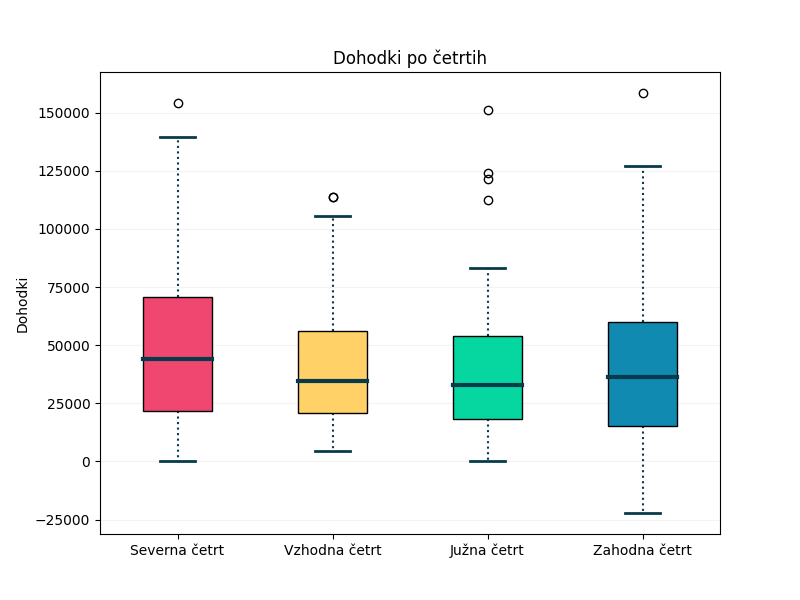
\includegraphics[scale=0.7]{Skatle_z_brki_Cetrti.png}
    \caption{Škatle z brki za dohodke po četrtih.}
    \label{brke_po_cetrtih}
\end{figure}

Najprej naredimo nekaj splošnih opazk.
Opazimo, da je variacija dohodkov znotraj severne in zahodne četrti nekoliko višja kot v vzhodni in južni četrti. 
Ker so prvi, drugi in tretji kvartil ter maksimum v severni četriti izmed vseh četrti največji, 
sklepamo, da je v povprečju dohodki v Severni četrti malenkost višji od ostalih. 
V vzhodni in južni četrti je porazdelitev nekoliko nagnjena k večjim dohodkom. 
Južna četrt ima največ osamelcev, dohodki pa so izmed vseh četrti najmanj razpršeni.

Na podlagi opaženega, sklepamo, da so dohodki v severni četrti nekoliko višji kot v ostalih.
Pravtako pa se zdi, da je varianca povprečnega dohodka med četrtmi relativno majhna.
Glede na to da smo iz vsake četrti izbrali zgolj $100$ vzorcev, populacija četrti pa je v povprečju $10.000$, ti podatki niso nujno reprezentativni.
Zato s tem sklepom postopamo previdno.

\subsection*{Primer (b)}

Iz severne četrti vzamemo še 4 vzorce velikosti $100$.
Tudi za te vzorce narišemo škatle z brki prikazane na sliki~\ref{brke_sever}.

\begin{figure}[H]
    \centering
    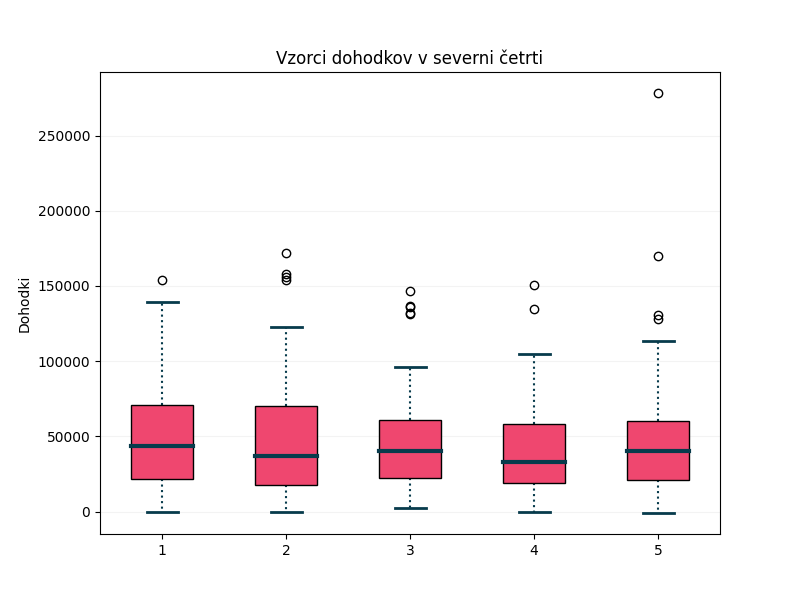
\includegraphics[scale=0.7]{Skatle_z_brki_Sever.png}
    \caption{Škatle z brki za dohodke v severni četrti.}
    \label{brke_sever}
\end{figure}

Mediane vseh škatel ležijo nad $40.000$, tako da sklepamo da večina dohodkov znaša več kot to.
Dohodki osamelcev znašaja v povprečju $150.000$.
Nasploh opazimo nekoliko več variacije med premožnejšimi prebivalci severne četriti.

\subsection*{Primer (c)}

Naj bo $N$ velikost populacije Kibergrada, $N_i$ velikost populacije $i$-te četrti in $w_i = N_i/N$ velikostni deleži četrti.
Nadaljnje naj bo $\mu_i$ povprečni dohodek in $\sigma_i^2$ varianca dohodka $i$-te četrti,
$\mu$ povprečni dohodek in $\sigma^2$ varianca dohodka celotne populacije ter $\sigma^2_p$ in $\sigma^2_n$ pojasnjena in nepojasnjena varianca celotne populacije.
Pojasnjeno in nepojasnjeno varianco pri stratificiranem vzorčenju lahko izrazimo kot
\[\sigma^2_p = \sum_{i=1}^4 w_i \mu_i^2 - \mu^2 \qquad \sigma^2_n = \sum_{i=1}^4 w_i \sigma_i^2.\]

Programa \textbf{naloga1.py} vrne, da pojasnjena varianca znaša, nepojasnjena varianca pa.
Nizka pojasnjena varianca potrjuje hipotezo, da je razlika povprečnega dohodka družine med četrtmi majhna. 

%%%%%%%%%%%%%%%%%%%%%%%%%%%%%%%%% - 2. naloga - %%%%%%%%%%%%%%%%%%%%%%%%%%%%%%%%%

\section*{2. naloga}

\subsection*{Primer (a)}

Najprej uvedimo nekaj oznak. 
Če je $k \in \set{1, \ldots, 12}$ število skokov ptic, naj bo $S_k$ frekvenca tega opažanja.
Podatke z novimi oznakami predstavimo v spodnji tabeli.
\begin{table}[H]
    \centering
    \begin{tabular}{|l|l|l|l|l|l|l|l|l|l|l|l|l|}
    \hline
    $k$ & 1 & 2 & 3 & 4 & 5 & 6 & 7 & 8 & 9 & 10 & 11 & 12 \\ \hline
    $S_k$ & 48 & 31 & 20 & 9 & 6 & 5 & 4 & 2 & 1 & 1 & 2 & 1 \\ \hline
    \end{tabular}
    \caption{Frekvence števila skokov}
    \label{freq}
\end{table}
Skupno število opaženih skokov označimo z $S$, število vseh opažanj pa z $N$.
Velja
\[N = \sum_{k=1}^{12} S_k \qquad S = \sum_{k=1}^{12} k S_k.\]
V našem primeru znaša $N = 130$ in $S = 363$.

Želimo poiskati geometrijsko porazdelitev, ki se najbolje prilega tem podatkom. 
Če je število skokov pri posameznem opažanju slučajna spremenljivka $K \sim \Geom(p)$, 
v resnici iščemo cenilko za parameter $p$.
To znamo narediti na vsaj dva načina.

\emph{Prvi način:} Postopamo po metodi momentov. 
Spomnimo se, da pričakovana vrednost geometrijske porazdelitve $\Geom(p)$ znaša $\frac{1}{p}$.
Zato velja
\[p = \frac{1}{E(K)}.\]
Po metodi momentov $\E(K)$ ocenimo s prvim momentom opaženih vrednosti 
\[\frac{1}{N} \sum_{k=1}^{12} k S_k = \frac{S}{N},\]
kar nam da cenilko
\[\hat{p} = \frac{N}{S}.\]

\emph{Drugi način:} Postopamo po metodi največjega verjetja.
Verjetnostna funkcija geometrijske porazdelitve $\Geom(p)$ je $\PP(K=k) = p(1-p)^{k-1}$.
Verjetje lahko torej izrazimo kot 
\[\Lver(p \mid S1, \ldots, S_{12}) = p^N (1-p)^{S - N}.\]
Ko logaritmiramo, dobimo 
\[\lver(p \mid S1, \ldots, S_{12}) = N \ln(\frac{p}{1-p}) + S \ln(1-p).\]
Če parcialno odvajamo po $p$ in malo računamo, ponovno pridemo do cenilke
\[\hat{p} = \frac{N}{S}.\]

V obeh primerih pridemo do iste cenilke.
Ta v našem primeru znaša 
\[\hat{p} = \frac{130}{363} \approx 0.358.\]
Teorija metode momentov in metode največjega verjetja nam zagotovita, da je ta izbira smiselna.
Iskana geometrijska porazdelitev je $\Geom(\hat{p})$.

\subsection*{Primer (b)}

Ob predpostavki, da je $K \sim \Geom(\hat{p})$, poračunamo verjetnosti $p_k$, da pri enem opažanju pride do $k$ skokov.
Pričakovano vrednosti frekvenc določimo kot
\[\hat{S}_k = p_k N.\]
Dobimo spodnjo tabelo.
\begin{table}[H]
    \centering
    \begin{tabular}{|c|c|c|c|c|c|c|}
    \hline
    $k$ & 1 & 2 & 3 & 4 & 5 & 6 \\ \hline
    $p_k$ & 0.3580 & 0.2298 & 0.1476 & 0.0947 & 0.0608 & 0.0390  \\ \hline
    $\hat{S}_k$ & 46.54 & 29.87 & 19.19 & 12.31 & 7.90 & 5.07 \\ \hline
    $k$ & 7 & 8 & 9 & 10 & 11 & 12 \\ \hline
    $p_k$ & 0.0251 & 0.0161 & 0.0103 & 0.0066 & 0.0043 & 0.0027 \\ \hline
    $\hat{S}_k$ & 3.26 & 2.09 & 1.34 & 0.86 & 0.56 & 0.35 \\ \hline
\end{tabular}
\caption{Pričakovane frekvence skokov.}
\label{PricakovaneFreq}
\end{table}
Te podatke združimo v spodnji črtni grafikon.
\begin{figure}[H]
    \centering
    \includegraphics[scale=0.8]{Črtni_grafikon.png}
    \caption{Črtni grafikon opaženih in pričakovanih prekvenc.}
\end{figure}


\subsection*{Primer (c)}

Izračunati moramo pričakovano vrednost naše cenilke.
Naj bo $K_i \sim \Geom(p)$ število skokov pri $i$-tem opažanju. Opazimo, da je
\[S = \sum_{i=1}^N K_i.\]
Če predpostavimo, da so spremenljivke $K_1, K_2, \ldots, K_N$ med sabo neodvisne, 
je slučajna spremenljivka $S$ porazdeljena negativno binomsko $\NegBin(N,p)$.
Računamo.
\[E(\hat{p}) = E(\frac{N}{S}) = \sum_{k=N}^{\infty} \frac{N}{k} \binom{k-1}{N-1}p^N(1-p)^{N-k}\]  





%%%%%%%%%%%%%%%%%%%%%%%%%%%%%%%%% - 3. naloga - %%%%%%%%%%%%%%%%%%%%%%%%%%%%%%%%%

\end{document}
